\section{Per-world demos}\label{per-world-demos}

\subsection{World 1: the game world of 2099}\label{world-1-the-game-world-of-2099}

\begin{center}\fbox{\begin{minipage}{0.94\linewidth}\setlength{\parskip}{4pt}\small

\textbf{Gap: world 1's demo.} One frame and a walk-through of every place of world 1, rendered from the stage the creator accepted for it. A first render of 9 October (5,292 frames on 20 rented L4 cards, 78 minutes, €15.82) is not shown, because its stages have changed since.

\end{minipage}}\end{center}

Figure A1 follows two objects through the stages, from the concept to the place.

\begin{figure}
\centering
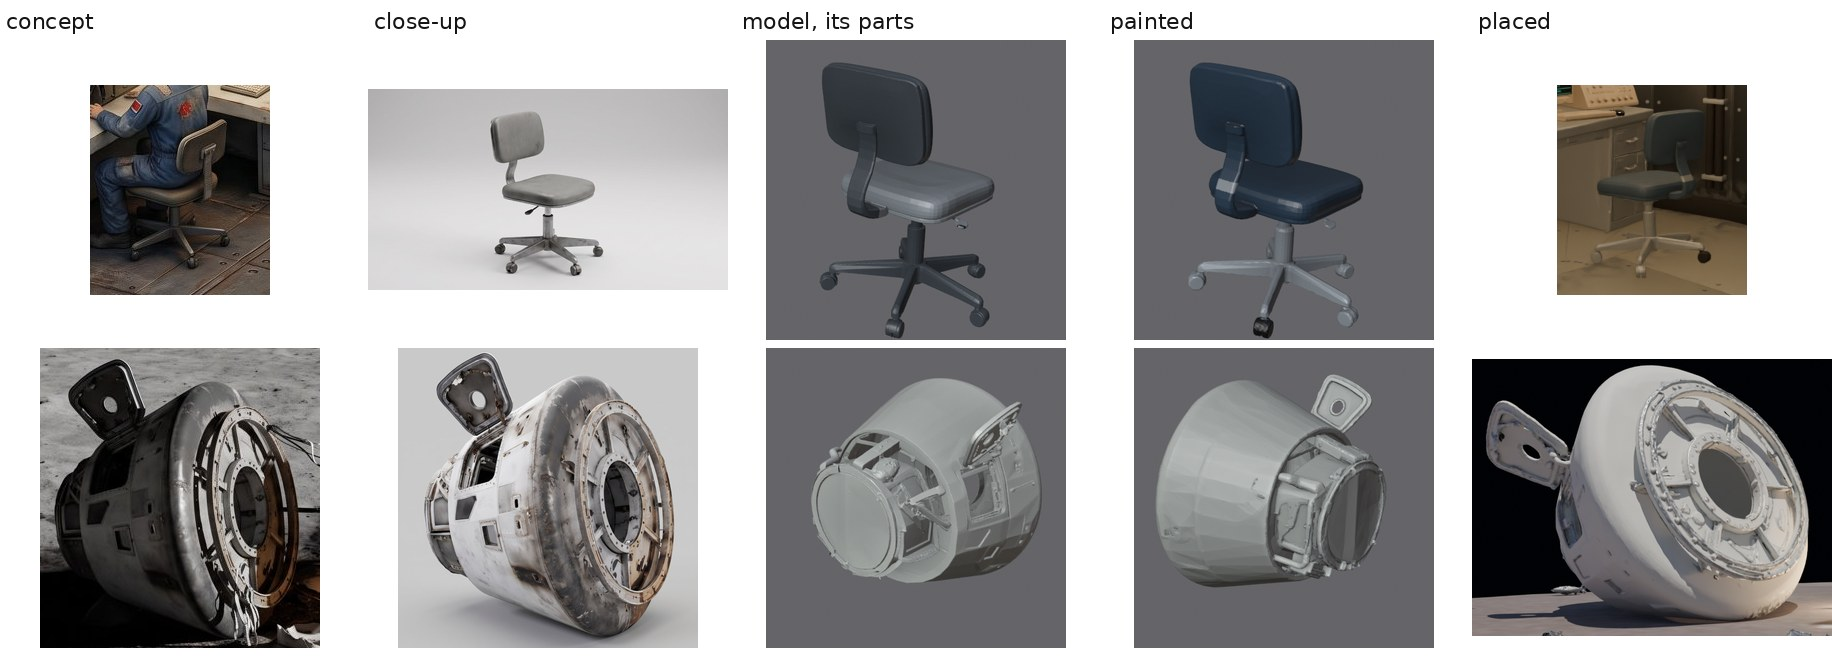
\includegraphics[width=1\linewidth,height=\textheight,keepaspectratio,alt={Two objects through the stages: the lab's desk chair (top) and the wreck's forward section (bottom). From left: the concept the creator chose, the close-up drawn from it, the generated model with its parts, the model painted from the surface library, and the model in its place on the stage. The forward section shows a known fault: its scorched paint has no part of its own and is lost in painting (Section 5).}]{figures/fig-stages.jpg}
\caption{Two objects through the stages: the lab's desk chair (top) and the wreck's forward section (bottom). From left: the concept the creator chose, the close-up drawn from it, the generated model with its parts, the model painted from the surface library, and the model in its place on the stage. The forward section shows a known fault: its scorched paint has no part of its own and is lost in painting (Section 5).}
\end{figure}

\begin{center}\fbox{\begin{minipage}{0.94\linewidth}\setlength{\parskip}{4pt}\small

\textbf{Gap: worlds 2 to 4, and a public link to the videos.} This appendix will show every place of the other three worlds in the same way. The videos of world 1 are not yet published at a public address.

\end{minipage}}\end{center}
